\section{Double Integrals in Polar Coordinates} \label{S:11.5.Double_Integrals_Polar}

\vspace*{-14 pt}
\framebox{\hspace*{3 pt}
\parbox{6.25 in}{\begin{goals}
\item What are the polar coordinates of a point in two-space?
\item How do we convert between polar coordinates and rectangular coordinates?
\item What is the area element in polar coordinates?
\item How do we convert a double integral in rectangular coordinates to a double integral in polar coordinates?
\end{goals}} \hspace*{3 pt}}


\subsection*{Introduction}

While we have naturally defined double integrals in the rectangular coordinate system, starting with domains that are rectangular regions, there are many of these integrals that are difficult, if not impossible, to evaluate.  For example, consider the domain $D$ that is the unit circle and $f(x,y) = e^{-x^2 - y^2}$.  To integrate $f$ over $D$, we would use the iterated integral
$$\iint_D f(x,y) \, dA = \int_{x = -1}^{x = 1} \int_{y = -\sqrt{1-x^2}}^{y = \sqrt{1-x^2}} e^{-x^2 - y^2} \, dy \, dx.$$
For this particular integral, regardless of the order of integration, we are unable to find an antiderivative of the integrand; in addition, even if we were able to find an antiderivative, the inner limits of integration involve relatively complicated functions.

It is useful, therefore, to be able to translate to other coordinate systems where the limits of integration and evaluation of the involved integrals is simpler.  In this section we provide a quick discussion of one such system -- polar coordinates -- and then introduce and investigate their ramifications for double integrals.  The rectangular coordinate system allows us to consider domains and graphs relative to a rectangular grid. The polar coordinate system is an alternate coordinate system that allows us to consider domains less suited to rectangular coordinates, such as circles.

\begin{pa} \label{PA:11.5}  The coordinates of a point determine its location. In particular, the rectangular coordinates of a point $P$ are given by an ordered pair $(x,y)$, where $x$ is the (signed) distance the point lies from the $y$-axis to $P$ and $y$ is the (signed) distance the point lies from the $x$-axis to $P$.  In polar coordinates, we locate the point by considering the distance the point lies from the origin, $(0,0)$, and the angle the line segment from the origin to $P$ forms with the positive $x$-axis.
    \ba
    \item Determine the rectangular coordinates of the following points:
        \begin{enumerate}[i.]
        \item The point $P$ that lies 1 unit from the origin on the positive $x$-axis.


        \item The point $Q$ that lies 2 units from the origin and such that $\overline{OQ}$ makes an angle of $\frac{\pi}{2}$ with the positive $x$-axis, where $O$ is the origin, $(0,0)$.


        \item The point $R$ that lies 3 units from the origin such that $\overline{OR}$ makes an angle of $\frac{2\pi}{3}$ with the positive $x$-axis.

        \end{enumerate}

    \item Part (a) indicates that the two pieces of information completely determine the location of a point:  either the traditional $(x,y)$ coordinates, or alternately, the distance $r$ from the point to the origin along with the angle $\theta$ that the line through the origin and the point makes with the positive $x$-axis. We write ``$(r, \theta)$'' to denote the point's location in its polar coordinate representation. Find polar coordinates for the points with the given rectangular coordinates.
        \begin{enumerate}[i.]
        \item $(0,-1)$  \hspace{1.0in} ii.  $(-2,0)$  \hspace{1.0in} iii.  $(-1,1)$

        \end{enumerate}

	\item For each of the following points whose coordinates are given in polar form, determine the rectangular coordinates of the point.
       \begin{enumerate}[i.]
          \item $(5, \frac{\pi}{4})$         \hspace{1.0in} ii. $(2, \frac{5\pi}{6})$   \hspace{1.0in} iii. $(\sqrt{3}, \frac{5\pi}{3})$
       \end{enumerate}

    \ea

\end{pa} 

\begin{activitySolution} 
   \ba
    \item Determine the rectangular coordinates of the following points:
        \begin{enumerate}[i.]
        \item This point has $y$ coordinate 0, so the $x$ coordinate must be 1 and the point is $(1,0)$.

        \item The angle of $\frac{\pi}{2}$ with the positive $x$-axis places the point on the $y$-axis. The point on the $y$-axis a distance 2 from the origin is the point $(0,2)$.

        \item Draw a right triangle from the origin to $R$ to the point on the $x$-axis below $R$. The acute angle at the origin has measure $\frac{\pi}{3}$. So $x = 3\cos\left(\frac{2\pi}{3}\right) = -\frac{3}{2}$ and $y = 3\sin\left(\frac{2\pi}{3}\right) = \frac{3\sqrt{3}}{2}$. So this point has rectangular coordinates $\left(-\frac{3}{2}, \frac{3\sqrt{3}}{2}\right)$.

        \end{enumerate}

    \item Part (a) indicates that the two pieces of information completely determine the location of a point:  either the traditional $(x,y)$ coordinates, or alternately, the distance $r$ from the point to the origin along with the angle $\theta$ that the line through the origin and the point makes with the positive $x$-axis. We write ``$(r, \theta)$'' to denote the point's location in its polar coordinate representation. Find polar coordinates for the points with the given rectangular coordinates.
        \begin{enumerate}[i.]
        \item The distance from the point with rectangular coordinates $(0,-1)$ to the origin is 1, and the angle the line through the origin and this point makes with the positive $x$-axis is $\frac{\pi}{2}$, so the polar coordinate representation of this point is $\left(1,\frac{\pi}{2}\right)$.

	\item The distance from the point with rectangular coordinates $(-2,0)$ to the origin is 2, and the angle the line through the origin and this point makes with the positive $x$-axis is $\pi$, so the polar coordinate representation of this point is $(2,\pi)$.

	\item The distance from the point with rectangular coordinates $(-1,1)$ to the origin is $\sqrt{2}$, and the angle the line through the origin and this point makes with the positive $x$-axis is $\frac{3\pi}{4}$, so the polar coordinate representation of this point is $\left(\sqrt{2},\frac{3\pi}{4}\right)$.


        \end{enumerate}

	\item For each of the following points whose coordinates are given in polar form, determine the rectangular coordinates of the point.
       \begin{enumerate}[i.]
          \item The rectangular coordinates are $x = 5 \cos\left(\frac{\pi}{4}\right) = \frac{5\sqrt{2}}{2}$ and $y = 5 \sin\left(\frac{\pi}{4}\right) = \frac{5\sqrt{2}}{2}$.
         \item  The rectangular coordinates are $x = 2 \cos\left(\frac{5\pi}{6}\right) = -\sqrt{3}$ and $y = 2 \sin\left(\frac{5\pi}{6}\right) = 1$.
		\item The rectangular coordinates are $x = \sqrt{3} \cos\left(\frac{5\pi}{3}\right) = \frac{\sqrt{3}}{2}$ and $y = \sqrt{3} \sin\left(\frac{5\pi}{3}\right) = -\frac{3}{2}$. 
       \end{enumerate}

    \ea


\end{activitySolution} 

\afterpa 

\subsection*{A Quick Overview of Polar Coordinates}

The rectangular coordinate system is best suited for graphs and regions that are naturally considered over a rectangular grid. The polar coordinate system is an alternative that offers good options for functions and domains that have more circular characteristics.  A point $P$ in rectangular coordinates that is described by an ordered pair $(x,y)$, where $x$ is the displacement from $P$ to the $y$-axis and $y$ is the displacement from $P$ to the $x$-axis, as seen in Preview Activity \ref{PA:11.5}, can also be described  with polar coordinates\index{polar coordinates} $(r,\theta)$, where $r$ is the distance from $P$ to the origin and $\theta$ is the angle formed by the line segment $\overline{OP}$ and the positive $x$-axis, as shown in Figure \ref{F:11.5.Polar_coords}.
\begin{figure}[ht]
\begin{center}
\begin{minipage}{2.5in}
\begin{center}
%\resizebox{!}{2.4in}{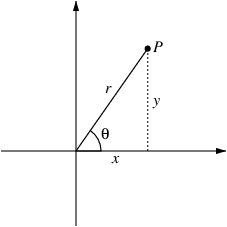
\includegraphics{11_5_Polar_coords}}
  
\includegraphics{figures/fig_11_5_polar_def.eps}
\end{center}
\caption{The polar coordinates of a point.}
\label{F:11.5.Polar_coords}
\end{minipage} \hspace{0.5in}
\begin{minipage}{2.5in}
\begin{center}
%\vspsace{0.05in}
%\resizebox{!}{2.4in}{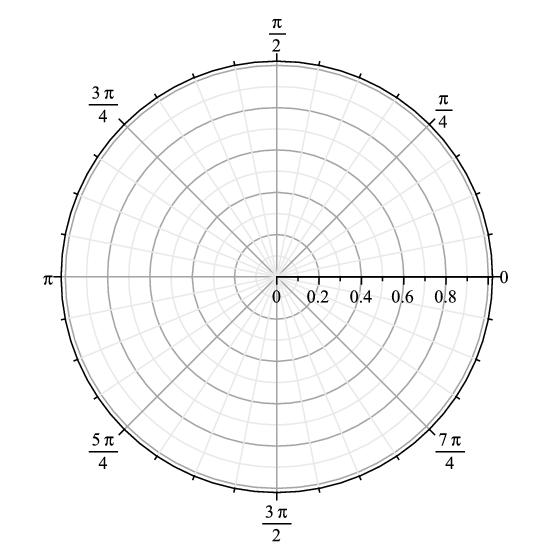
\includegraphics{11_5_Polar_grid}}
  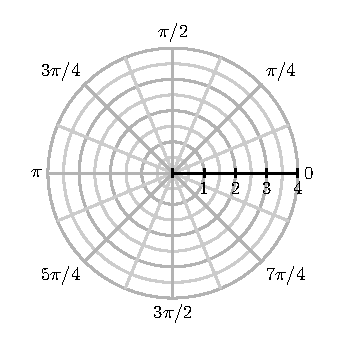
\includegraphics{figures/fig_11_5_polar_grid.eps}
\end{center}
\caption{The polar coordinate grid.}
\label{F:11.5.Polar_grid}
\end{minipage}
\end{center}
\end{figure}
Trigonometry and the Pythagorean Theorem allow for straightforward conversion from rectangular to polar, and vice versa.

 \vspace*{5pt}
\nin \framebox{\hspace*{3 pt}
\parbox{6.25 in}{\begin{description}
\item[Converting from rectangular to polar.] If we are given the rectangular coordinates $(x,y)$ of a point $P$, then the polar coordinates $(r,\theta)$ of $P$ satisfy
\[r = \sqrt{x^2+y^2} \ \ \ \ \ \text{ and } \ \ \ \ \ \tan(\theta) = \frac{y}{x}, \text{ assuming } x \neq 0.\]
\item[Converting from polar to rectangular.] If we are given the polar coordinates $(r,\theta)$ of a point $P$, then the rectangular coordinates $(x,y)$ of $P$ satisfy
\[x = r\cos(\theta)  \ \ \ \ \ \text{ and } \ \ \ \ \ y = r\sin(\theta).\]
\end{description}
} \hspace*{3 pt}}
\vspace*{5pt}

%\begin{activity} \label{A:11.5.1} \ba
	\item Find the rectangular coordinates of the point whose polar coordinates are $\left(2, -\frac{\pi}{3}\right)$.



	\item Find polar coordinates for the point whose rectangular coordinates are $P=(-1, 1)$. Now find a second pair of polar coordinates for the point $P$. How many different ways are there to represent a point in polar coordinates?
	
	
	
	\ea

\end{activity}
\begin{smallhint}

\end{smallhint}
\begin{bighint}

\end{bighint}
\begin{activitySolution}
\ba
	\item We have $r = 2$ and $\theta = -\frac{\pi}{3}$, so 
\[x = 2 \cos\left(-\frac{\pi}{3}\right) = 1 \ \text{ and } \ y = 2 \sin\left(-\frac{\pi}{3}\right) = -\sqrt{3}.\]

	\item Since $x = -1$ and $y = 1$ we have $r = \sqrt{(-1)^1 + 1^2} = \sqrt{2}$. The point $(-1,1)$ is in the second quadrant, and $\tan(\theta) = -1$, so $\theta = \frac{3\pi}{4}$. We can also use any angle for $\theta$ that is co-terminal with $\frac{3\pi}{4}$, so $\left(\sqrt{2}, \frac{3\pi}{4} + 2k \pi\right)$ is a set of polar coordinates for $(-1,1)$ for any integer $k$. This shows that we can represent the same point in infinitely many different ways in polar coordinates. 
	
	\ea
\end{activitySolution}
\aftera


We can draw graphs of curves in polar coordinates in a similar way to how we do in rectangular coordinates. However, when plotting in polar coordinates, we use a grid that considers changes in angles and changes in distance from the origin.  In particular,  the angles $\theta$ and distances $r$ partition the plane into small wedges as shown in Figure \ref{F:11.5.Polar_grid}.

\begin{activity} \label{A:11.5.2} Most polar graphing devices\footnote{You can use your calculator in POL mode, or a web applet such as \url{http://webspace.ship.edu/msrenault/ggb/polar_grapher.html}} can plot curves in polar coordinates of the form $r = f(\theta)$. Use such a device to complete this activity.
	\ba
	\item Before plotting the polar curve $r=1$, think about what shape it should have, in light of how $r$ is connected to $x$ and $y$. Then use appropriate technology to draw the graph and test your intuition.

	\item The equation $\theta = 1$ does not define $r$ as a function of $\theta$, so we can't graph this equation on many polar plotters. What do you think the graph of the polar curve $\theta = 1$ looks like? Why?
	
	\item Before plotting the polar curve $r = \theta$, what do you think the graph looks like? Why? Use technology to plot the curve and compare your intuition.

         \item What about the curve $r = \sin(\theta)$?  After plotting this curve, experiment with others of your choosing and think about why the curves look the way they do.	
    	
	\ea

\end{activity}
\begin{smallhint}

\end{smallhint}
\begin{bighint}

\end{bighint}
\begin{activitySolution}
	\ba
	\item Since $r$ represents a distance from the origin, any curve with a constant value of $r$ should be a circle, centered at the origin, with radius $r$. 

	\item The set of points with a constant value of $\theta$ all make the same angle with the positive $x$-axis. This set of points should then form a line through the origin making an angle $\theta$ with the positive $x$-axis.  
		
	\item As $\theta$ increases, so does the value of $r$. Thus, as the point $(r,r)$ rotates around the origin, its distance from the origin also increases in a uniform manner. The set of these points should be a spiral, spiraling away from the origin as it rotates counterclockwise around the origin. 	

    \item As $\theta$ increases, the values of $r$ will oscillate between $-1$ and $1$. When $r$ is negative, we reflect around the origin. So the resulting curve should look like a circle in the first and second quadrants. Note that $r=\sin(\theta)$ can also be represented as $r^2 = r\sin(\theta)$. So in rectangular coordinates the curve $r=\sin(\theta)$ has equation $x^2+y^2 = y$, or $x^2 + \left(y-\frac{1}{2}\right)^2 = \frac{1}{4}$. This is a circle  centered at $\left(0,frac{1}{2}\right)$ with radius $\frac{1}{2}$.   

    	
	\ea
\end{activitySolution}
\aftera



\subsection*{Integrating in Polar Coordinates}

Consider the double integral
\[\iint_D e^{x^2+y^2} \, dA,\]
where $D$ is the unit disk.  While we cannot directly evaluate this integral in rectangular coordinates,  a change to polar coordinates will convert it to one we can easily evaluate.

We have seen how to evaluate a double integral $\displaystyle \iint_D f(x,y) \, dA$ as an iterated integral of the form
\[\int_a^b \int_{g_1(x)}^{g_2(x)} f(x,y) \, dy \, dx\]
in rectangular coordinates, because we know that $dA = dy \, dx$ in rectangular coordinates. To make the change to polar coordinates, we not only need to represent the variables $x$ and $y$ in polar coordinates, but we also must understand how to write the area element, $dA$, in polar coordinates. That is, we must determine how the area element $dA$ can be written in terms of $dr$ and $d\theta$ in the context of polar coordinates.  We address this question in the following activity.

\begin{figure}[ht]
\begin{center}
\begin{minipage}{2.5in}
\begin{center}
%\resizebox{!}{2.4in}{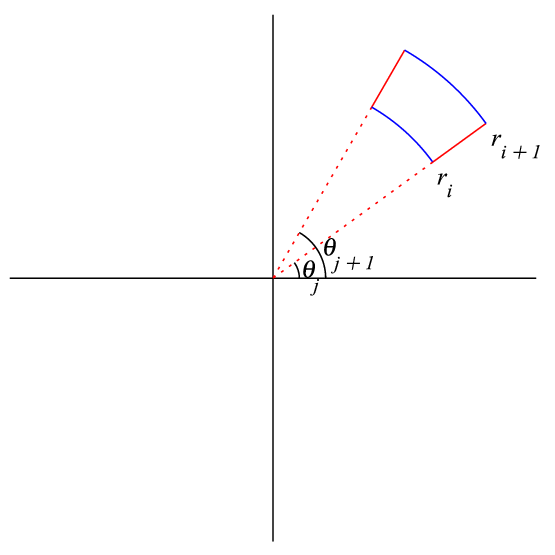
\includegraphics{11_5_Polarelement}}
  
\includegraphics{figures/fig_11_5_polar_rect.eps}
\end{center}
\caption{A polar rectangle.}
\label{F:11.5.Polar_area_a}
\end{minipage} \hspace{0.5in}
\begin{minipage}{2.5in}
\begin{center}
%\resizebox{!}{2.4in} {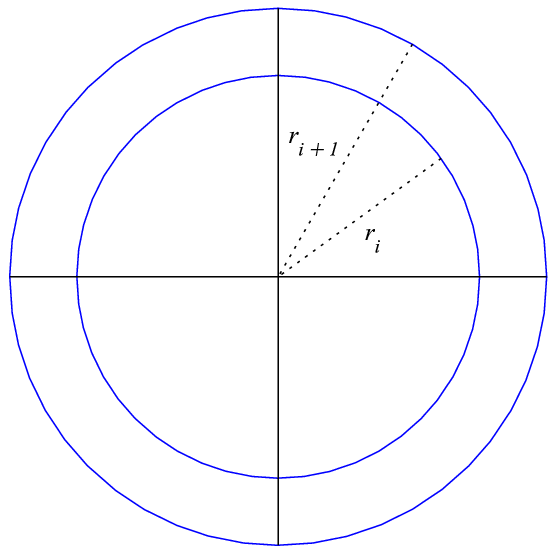
\includegraphics{11_5_Polarannulus}}
  
\includegraphics{figures/fig_11_5_annulus.eps}
\end{center}
\caption{An annulus.}
\label{F:11.5.Polar_area_b}
\end{minipage}
\end{center}
\end{figure}

\begin{activity} \label{A:11.5.3} Consider a polar rectangle $R$, with $r$ between $r_i$ and $r_{i+1}$ and $\theta$ between $\theta_j$ and $\theta_{j+1}$ as shown in Figure \ref{F:11.5.Polar_area_a}. Let $\Delta r = r_{i+1}-r_i$ and $\Delta \theta = \theta_{j+1}-\theta_j$. Let $\Delta A$ be the area of this region.
	\ba
	\item Explain why the area $\Delta A$ in polar coordinates is not $\Delta r \, \Delta \theta$.



	\item Now find $\Delta A$ by the following steps:
		\begin{enumerate}[i.]
		\item Find the area of the annulus (the washer-like region) between $r_i$ and $r_{i+1}$, as shown at right in Figure \ref{F:11.5.Polar_area_b}. This area will be in terms of $r_i$ and $r_{i+1}$.

		\item Observe that the region $R$ is only a portion of the annulus, so the area $\Delta A$ of $R$ is only a fraction of the area of the annulus.  For instance, if $\theta_{i+1} - \theta_i$ were $\frac{\pi}{4}$, then the resulting wedge would be 
		$$\frac{ \frac{\pi}{4} }{2\pi} = \frac{1}{8}$$
		of the entire annulus.  In this more general context, using the wedge between the two noted angles, what fraction of the area of the annulus is the area $\Delta A$? 

		\item Write an expression for $\Delta A$ in terms of $r_i$, $r_{i+1}$, $\theta_j$, and $\theta_{j+1}$.

		\item Finally, write the area $\Delta A$ in terms of $r_i$, $r_{i+1}$, $\Delta r$, and $\Delta \theta$, where each quantity appears only once in the expression. (Hint: Think about how to factor a difference of squares.)
	

	
		\end{enumerate}
	
	\item As we take the limit as $\Delta r$ and $\Delta \theta$ go to 0, $\Delta r$ becomes $dr$, $\Delta \theta$ becomes $d \theta$, and $\Delta A$ becomes $dA$, the area element. Using your work in (iv), write $dA$ in terms of $r$, $dr$, and $d \theta$.



	\ea

\end{activity}
\begin{smallhint}

\end{smallhint}
\begin{bighint}

\end{bighint}
\begin{activitySolution}
	\ba
	\item The quantity $\Delta r \, \Delta \theta$ would be the area of a rectangle with side lengths $\Delta r$ and $\Delta \theta$. The area $\Delta A$ of the polar region is the area of a slice of a washer, not a rectangle -- the sides are not all straight. 

	\item Now find $\Delta A$ by following these steps.
		\begin{enumerate}[i.]
		\item The area of the annulus between $r_i$ and $r_{i+1}$ is the area of the disk with larger radius $r_{i+1}$ minus the area of the disk with smaller radius $r_{i}$. So the area of the annulus is $\pi r^2_{i+1} - \pi r^2_{i}$. 

		\item Our region $R$ is the portion of the annulus between $\theta_{i}$ and $\theta_{i+1}$. So the angle that cuts the region $R$ from the annulus has measure $\Delta \theta = \theta_{i+1} - \theta_{i}$. Since the central angle of the entire annulus is $2 \pi$, the area of the region $R$ is the fractional portion $\frac{\Delta \theta}{2 \pi}$ of the whole annulus. 

		\item The fractional portion $\frac{\Delta \theta}{2 \pi}$ of the area of the whole annulus is 
\[\Delta A = \frac{\Delta \theta}{2 \pi} \left( \pi r^2_{i+1} - \pi r^2_{i} \right).\]

		\item Using a difference of squares gives us
\begin{align*}
\Delta A &= \frac{\Delta \theta}{2 \pi} \left( \pi r^2_{i+1} - \pi r^2_{i} \right) \\
	&= \frac{1}{2}\Delta \theta (r_{i+1} +  r_{i})(r_{i+1} -  r_{i}) \\
	&= \frac{1}{2}(r_{i+1} +  r_{i}) \Delta \theta  \Delta r.
\end{align*}
		
		\end{enumerate}
	
	\item Taking the limit as $\Delta r$ and $\Delta \theta$ go to 0, both $r_{i+1}$ and $r_i$ approach the same value $r$, so 
\[dA = \frac{1}{2}(r+r) \, dr \, d \theta = r \, dr \, d \theta.\]

	\ea
\end{activitySolution}
\aftera



From the result of Activity \ref{A:11.5.3}, we see when we convert an integral from rectangular coordinates to polar coordinates, we must not only convert $x$ and $y$ to being in terms of $r$ and $\theta$, but we also have to change the area element to $dA = r \, dr \, d\theta$ in polar coordinates. In other words, given a double integral $\iint_D f(x,y) \, dA$ in rectangular coordinates, to write a corresponding iterated integral in polar coordinates, we replace $x$ with $r \cos(\theta)$, $y$ with $r \sin(\theta)$ and $dA$ with $r \, dr \, d\theta$. Of course, we need to describe the region $D$ in polar coordinates as well. To summarize:

 \vspace*{5pt}
\nin \framebox{\hspace*{3 pt}
\parbox{6.25 in}{The double integral $\iint_D f(x,y) \, dA$ in rectangular coordinates can be converted to a double integral in polar coordinates\index{iterated integral!polar coordinates} as $\iint_D f(r\cos(\theta), r\sin(\theta)) \, r \, dr \, d\theta$.
} \hspace*{3 pt}}
\vspace*{5pt}


\begin{example} Let $f(x,y) = e^{x^2+y^2}$ on the disk $D = \{(x,y) : x^2 + y^2 \leq 1\}$.  We will evaluate $\iint_D f(x,y) \, dA$.

In rectangular coordinates the double integral $\ds \iint_D f(x,y) \, dA$ can be written as the iterated integral
\[\ds \iint_D f(x,y) \, dA = \int_{x=-1}^{x=1} \int_{y=-\sqrt{1-x^2}}^{y=\sqrt{1-x^2}} e^{x^2+y^2} \, dy \, dx.\]
We cannot evaluate this iterated integral, because $e^{x^2 + y^2}$ does not have an elementary antiderivative with respect to either $x$ or $y$.  However, since $r^2=x^2+y^2$ and the region $D$ is circular, it is natural to wonder whether converting to polar coordinates will allow us to evaluate the new integral. To do so, we replace $x$ with $r \cos(\theta)$, $y$ with $r \sin(\theta)$, and $dy \, dx$ with $r \, dr \, d\theta$ to obtain
\[\ds \iint_D f(x,y) \, dA = \iint_D e^{r^2} \, r \, dr \, d\theta.\]
The disc $D$ is described in polar coordinates by the constraints $0 \leq r \leq 1$ and $0 \leq \theta \leq 2\pi$.  Therefore, it follows that
\[\iint_D e^{r^2} \, r \, dr \, d\theta = \int_{\theta=0}^{\theta = 2\pi} \int_{r=0}^{r=1} e^{r^2} \, r \, dr \, d\theta.\]
We can evaluate the resulting iterated polar integral as follows:
\begin{align*}
\int_{\theta=0}^{\theta = 2\pi} \int_{r=0}^{r=1} e^{r^2} \, r \, dr \, d\theta &= \int_{\theta=0}^{2\pi}  \left( \frac{1}{2}e^{r^2}\biggm|_{r=0}^{r=1} \right) \, d\theta \\
	&= \frac{1}{2} \int_{\theta=0}^{\theta = 2\pi} \left( e-1 \right) \, d\theta \\
	&= \frac{1}{2}(e-1) \int_{\theta=0}^{\theta = 2\pi} \, d\theta \\
	&= \frac{1}{2}(e-1)\left[\theta\right]\biggm|_{\theta=0}^{\theta = 2\pi} \\
	&= \pi(e-1).
\end{align*}
\end{example}

While there is no firm rule for when polar coordinates can or should be used, they are a natural alternative anytime the domain of integration may be expressed simply in polar form, and/or when the integrand involves expressions such as $\sqrt{x^2 + y^2}.$

\begin{activity} \label{A:11.5.4} Let $f(x,y) = x+y$ and $D = \{(x,y) : x^2 + y^2 \leq 4\}$.
    \ba
    \item Write the double integral of $f$ over $D$ as an iterated integral in rectangular coordinates.

    \item Write the double integral of $f$ over $D$ as an iterated integral in polar coordinates.

    \item Evaluate one of the iterated integrals. Why is the final value you found not surprising?


    \ea


\end{activity}
\begin{smallhint}

\end{smallhint}
\begin{bighint}

\end{bighint}
\begin{activitySolution}
    \ba
    \item The integral $\ds \int \int_D f(x,y) \, dA$ can be written as the iterated integral
\[\int_{x=-2}^{2} \int_{y=-\sqrt{4-x^2}}^{\sqrt{4-x^2}} x+y \, dy \, dx.\]

    \item To convert to polar coordinates, we replace $x$ with $r \cos(\theta)$, $y$ with $r \sin(\theta)$ and $dy \ dx$ with $r \, dr \, d\theta$ to obtain
\[\int \int_D \left[ r \cos(\theta) + r \sin(\theta) \right] \ r \, dr \, d\theta.\]
The disc $D$ is described in polar coordinates by the constraints $0 \leq r \leq 2$ and $0 \leq \theta \leq 2\pi$. So we have
\[\int \int_D r\cos(\theta) + r \sin(\theta) \ r \, dr \, d\theta = \int_{\theta=0}^{2\pi} \int_{r=0}^2 \left[r\cos(\theta) + r \sin(\theta)\right] \ r \, dr \, d\theta.\]

    \item We evaluate the integral in polar coordinates as follows:
\begin{align*}
\int_{\theta=0}^{2\pi} \int_{r=0}^2 \left[r\cos(\theta) + r \sin(\theta)\right] \ r \, dr \, d\theta &= \int_{\theta=0}^{2\pi} \int_{r=0}^2 r^2\left[\cos(\theta) + \sin(\theta)\right] \, dr \, d\theta \\
	&= \int_{\theta=0}^{2\pi} \left( \left[\cos(\theta) + \sin(\theta)\right]\frac{r^3}{3}\biggm|_{r=0}^2 \right) \, d\theta \\
	&= \int_{\theta=0}^{2\pi} \frac{8}{3} \left[ \cos(\theta) + \sin(\theta) \right] \, d\theta \\
	&= \frac{8}{3}\left[\sin(\theta) - \cos(\theta)\right]\biggm|_{\theta=0}^{2\pi} \\
	&= \frac{8}{3}[(-1)-(-1)] \\
	&= 0.
\end{align*}
The graph of the plane $z=x+y$ crosses the $xy$-plane along the line $y=-x$, and bounds the same amount of volume below the $xy$-plane as above on the disk $D$. So we should have expected the value of the integral to be $0$.

    \ea
\end{activitySolution}
\aftera


\begin{figure}[ht]
\begin{center}
%\resizebox{!}{1.5in}{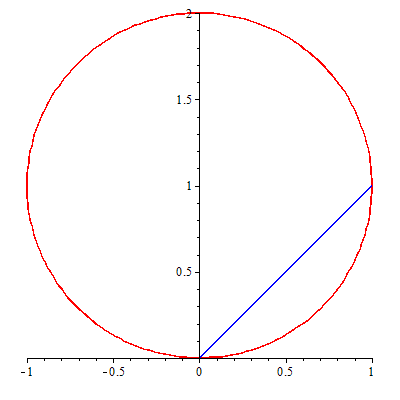
\includegraphics{11_5_Polar_ex2}}
  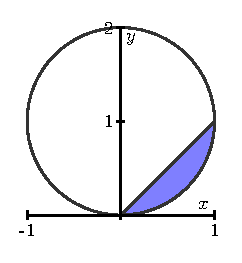
\includegraphics{figures/fig_11_5_polar_region.eps}
\end{center}
\caption{The graphs of $y=x$ and $x^2 + (y-1)^2 = 1$, for use in Activity~\ref{A:11.5.5}.}
\label{F:11.5.Polar_exercise}
\end{figure}

\newpage

\begin{activity} \label{A:11.5.5} 
Consider the circle given by $x^2 + (y-1)^2 = 1$ as shown in Figure \ref{F:11.5.Polar_exercise}.

\ba
	\item Determine a polar curve in the form $r = f(\theta)$ that traces out the circle $x^2 + (y-1)^2 = 1$.
	\item Find the exact average value of $g(x,y) = \sqrt{x^2 + y^2}$ over the interior of the circle $x^2 + (y-1)^2 = 1$.
	\item Find the volume under the surface $h(x,y) = x$ over the region $D$, where $D$ is the region bounded above by the line $y=x$ and below by the circle.
	\item Explain why in both (b) and (c) it is advantageous to use polar coordinates. 
\ea



\end{activity}
\begin{smallhint}

\end{smallhint}
\begin{bighint}

\end{bighint}
\begin{activitySolution}
\ba
\item When expanded, the equation of the circle is $x^2+y^2 - 2y = 0$. We can write this in polar coordinates as $r^2 - 2r \sin(\theta) = 0$, or $r = 2\sin(\theta)$.  Thus, the circle $C$ can be described as $0 \leq r \leq \ 2\sin(\theta)$ with $0 \leq \theta \leq \pi$. 

\item The circle $C$ has radius 1, so $A(C) = \pi$. Note that $g(x,y) = \sqrt{x^2 + y^2}$ can be written in polar form as $g(r,\theta) = r$. Thus, the average value of $g$ over $C$ is 
\begin{align*}
\frac{1}{\pi}\int \int_C g(x,y) \, dA &= \int_{0}^{\pi} \int_{0}^{2\sin(\theta)} r r \, dr \, d \theta \\
	&= \frac{1}{\pi}\int_{0}^{\pi} \frac{r^3}{3} \biggm|_{0}^{2\sin(\theta)} \, d \theta \\
	&= \frac{8}{3\pi} \int_{0}^{\pi} \sin^3(\theta) \, d \theta \\
	&= \frac{8}{3\pi} \int_{0}^{\pi} \sin(\theta)(1-\cos^2(\theta)) \, d \theta \\
	&= \frac{8}{3\pi} \left(-\cos(\theta)+\frac{\cos^3(\theta)}{3}\right)\biggm|_{0}^{\pi}   \\
	&= \frac{8}{3\pi}\left(2-\frac{2}{3}\right) \\
	&= \frac{32}{9\pi}.
\end{align*}

\item In polar coordinates, the line $y=x$ is represented as $r \sin(\theta) = r \cos(\theta)$, or $\tan(\theta) = 1$, or $\theta = \frac{\pi}{4}$. Therefore, the region $D$ is described by $0 \leq r \leq \ 2\sin(\theta)$ with $0 \leq \theta \leq \pi/4$. So the under the surface $h(x,y) = x$ over the region $D$ is given by
\begin{align*}
\int \int_D x \, dA &= \int_{0}^{\pi/4} \int_{0}^{2\sin(\theta)} r\cos(\theta) r \, dr \, d \theta \\
	&= \int_{0}^{\pi/4} \cos(\theta) \frac{r^3}{3} \biggm|_{0}^{2\sin(\theta)} \, d \theta \\
	&= \frac{8}{3} \int_{0}^{\pi/4} \cos(\theta) \sin^3(\theta) \, d \theta \\
	&= \frac{8}{12} \left. \sin^4(\theta) \right|_{0}^{\pi/4}  \\
	&= \frac{2}{3} \left(\frac{\sqrt{2}}{2}\right)^4  \\
	&= \frac{1}{6}.
\end{align*} 

\item In (b), it is very difficult to integrate $\sqrt{x^2+y^2}$ in rectangular coordinates, and in (c) the region $D$ is much more easily described in polar coordinates. 

\ea

\end{activitySolution}
\aftera



\begin{summary}
\item The polar representation of a point $P$ is the ordered pair $(r,\theta)$ where $r$ is the distance from the origin to $P$ and $\theta$ is the angle the ray through the origin and $P$ makes with the positive $x$-axis.
\item The polar coordinates $r$ and $\theta$ of a point $(x,y)$ in rectangular coordinates satisfy
\[r = \sqrt{x^2+y^2} \ \ \ \ \ \text{ and } \ \ \ \ \ \tan(\theta) = \frac{y}{x};\]
the rectangular coordinates $x$ and $y$ of a point $(r,\theta)$ in polar coordinates satisfy
\[x = r\cos(\theta)  \ \ \ \ \ \text{ and } \ \ \ \ \ y = r\sin(\theta).\]
\item The area element $dA$ in polar coordinates is determined by the area of a slice of an annulus and is given by
\[dA = r \, dr \, d\theta.\]
\item To convert the double integral ${\iint_D f(x,y) \, dA}$ to an iterated integral in polar coordinates, we substitute $r \cos(\theta)$ for $x$, $r \sin(\theta)$ for $y$, and $r \, dr \, d\theta$ for $dA$ to obtain the iterated integral 
\[{\iint_D f(r\cos(\theta), r\sin(\theta)) \, r \, dr \, d\theta}.\]
\end{summary}

\nin \hrulefill

\begin{exercises} 

\item Consider the iterated integral $I = \ds \int_{-3}^{0} \int_{-\sqrt{9-y^2}}^{0} \frac{y}{x^2 + y^2+1} \, dx \, dy.$  
	
\ba
	\item Sketch (and label) the region of integration.
	\item Convert the given iterated integral to one in polar coordinates.
	\item Evaluate the iterated integral in (b).
	\item State one possible interpretation of the value you found in (c).
\ea

\begin{exerciseSolution}
\ba
	\item The region $R$ defined by $-\sqrt{9-y^2} \leq x \leq 0$ and $-3 \leq y \leq 0$ is the portion of the circle centered at the origin of radius 3 that is in the third quadrant. 
	\item The region $R$ is described in polar coordinates by $0 \leq r \leq 3$ and $\pi \leq \theta \leq \frac{3 \pi}{2}$. With $r^2=x^2+y^2$ and $y = r\sin(\theta)$ we have  
\[\int_{-3}^{0} \int_{-\sqrt{9-y^2}}^{0} \frac{y}{x^2 + y^2+1} \, dx \, dy = \int_{\pi}^{3\pi/2} \int_{0}^{3} \frac{r\sin(\theta)}{r^2+1} r \, dr \, d\theta.\]

	\item Dividing $1+r^2$ into $r^2$ shows that $\frac{r^2}{r^2+1} = 1 - \frac{1}{r^2+1}$. Using this fact gives us 
\begin{align*}
\int_{\pi}^{3\pi/2} \int_{0}^{3} \frac{r^2\sin(\theta)}{r^2+1} \, dr \, d\theta &= \int_{\pi}^{3\pi/2} \sin(\theta) \int_{0}^{3} \frac{r^2}{r^2+1} \, dr \, d\theta \\
	&= \int_{\pi}^{3\pi/2} \sin(\theta) \int_{0}^{3} 1-\frac{1}{r^2+1} \, dr \, d\theta \\
	&= \int_{\pi}^{3\pi/2} \sin(\theta)  \left(r-\arctan(r)\right)\biggm|_{0}^{3} \, d\theta \\
	&= \int_{\pi}^{3\pi/2} \sin(\theta)  \left(3-\arctan(3)\right) \, d\theta \\
	&= \left(3-\arctan(3)\right) (-\cos(\theta))\biggm|_{\pi}^{3\pi/2}	 \\
	&= \arctan(3)-3.
\end{align*}
 
	\item If $f(x,y) = \frac{y}{x^2 + y^2+1}$ is the density of the lamina defined by $R$, then $I$ represents the mass of the lamina.
\ea
\end{exerciseSolution}

\item Let $D$ be the region that lies inside the unit circle in the plane.
	
\ba
	\item Set up and evaluate an iterated integral in polar coordinates whose value is the area of $D$.
	\item Determine the exact average value of $f(x,y) = y$ over the upper half of $D$.
	\item Find the exact center of mass of the lamina over the portion of $D$ that lies in the first quadrant and has its mass density distribution given by $\delta(x,y) = 1$. (Before making any calculations, where do you expect the center of mass to lie? Why?)
	\item Find the exact volume of the solid that lies under the surface $z = 8-x^2-y^2$ and over the unit disk, $D$.
\ea

\begin{exerciseSolution}
\ba
	\item The unit disk $D$ is described in polar coordinates as $0 \leq r \leq 1$ and $0 \leq \theta \leq 2 \pi$. So an iterated integral in polar coordinates whose value is the area of $D$ is 
	\[\int_{0}^{2 \pi} \int_{0}^{1} r \, dr \, d\theta.\]
	
	\item The upper half $H$ of $D$ is represented by restricting $\theta$ to $0 \leq \theta \leq \pi$. Since the area of this half-disk is $\pi$, the exact average value of $f(x,y) = y$ over the upper half of $D$ is
	\begin{align*}
	\frac{1}{\pi} \iint_H f(x,y) \, dA &=  \int_{0}^{\pi} \int_{0}^{1} r (r\sin(\theta)) \, dr \, d\theta \\
		&= \frac{1}{\pi} \int_{0}^{\pi} \sin(\theta) \frac{1}{3}r^3\biggm|_{0}^{1} \, d\theta \\
		&= \frac{1}{3 \pi} \int_{0}^{\pi} \sin(\theta) \, d\theta \\
		&= \frac{1}{3 \pi} (-\cos(\theta))\biggm|_{0}^{\pi} \\
		&= \frac{2}{3\pi}.
	\end{align*}
	
	\item The region and density function are symmetric around the line $y=x$, so we should expect the center of mass to lie on this line. The inequalities $0 \leq \theta \leq \frac{\pi}{2}$ describe the first quadrant region $Q$ of $D$. The area of $Q$ is $\frac{\pi}{2}$. The center of mass $(\overline{x}, \overline{y})$ of this region with mass density distribution given by $\delta(x,y) = 1$ is found by 
\begin{align*}
\overline{x} &= \frac{2}{\pi} \int_{0}^{\pi/2} \int_{0}^{1} r(r \cos(\theta)) \, dr \, d\theta \\
		&= \frac{2}{\pi} \int_{0}^{\pi/2} \cos(\theta) \frac{1}{3}r^3\biggm|_{0}^{1} \, d\theta \\
		&= \frac{2}{3 \pi} \int_{0}^{\pi/2} \cos(\theta) \, d\theta \\
		&= \frac{2}{3 \pi} (\sin(\theta))\biggm|_{0}^{\pi/2} \\
		&= \frac{2}{3\pi}
	\end{align*}
and
	\begin{align*}
\overline{y} &=  \frac{2}{\pi} \int_{0}^{\pi/2} \int_{0}^{1} r (r\sin(\theta)) \, dr \, d\theta \\
		&= \frac{2}{\pi} \int_{0}^{\pi/2} \sin(\theta) \frac{1}{3}r^3\biggm|_{0}^{1} \, d\theta \\
		&= \frac{2}{3 \pi} \int_{0}^{\pi/2} \sin(\theta) \, d\theta \\
		&= \frac{2}{3 \pi} (-\cos(\theta))\biggm|_{0}^{\pi/2} \\
		&= \frac{2}{3\pi}.
	\end{align*}

	\item The volume is 
\begin{align*}
\iint_D 8-x^2-y^2 \, dA &= \int_{0}^{2\pi} \int_0^1 (8-r^2) r \, dr \, d \theta \\
	&= \int_{0}^{2\pi} \left( 4r^2 -\frac{1}{4}r^4 \right)\biggm|_0^1 \, d \theta \\
	&= \frac{15}{4} \int_{0}^{2\pi} \, d \theta \\
	&= \frac{15 \pi}{2}. 
\end{align*}

\ea
\end{exerciseSolution}


\item For each of the following iterated integrals, (a) sketch and label the region of integration, (b) convert the integral to the other coordinate system (if given in polar, to rectangular; if given in rectangular, to polar), and (c) choose one of the two iterated integrals to evaluate exactly.
	
\ba
	\item $\ds \int_{\pi}^{3\pi/2} \int_{0}^{3}  r^3 \, dr \, d\theta$
	\item $\ds \int_{0}^{2} \int_{-\sqrt{1-(x-1)^2}}^{\sqrt{1-(x-1)^2}} \sqrt{x^2 + y^2} \, dy \, dx$ 
	\item $\ds \int_0^{\pi/2} \int_0^{\sin(\theta)} r \sqrt{1-r^2} \, dr \, d\theta.$
	\item $\ds \int_0^{\sqrt{2}/2} \int_y^{\sqrt{1-y^2}} \cos(x^2 + y^2) \, dx \, dy.$
\ea

\begin{exerciseSolution}
\ba
	\item The region is the third quadrant portion of the disk centered at the origin of radius 3. In rectangular coordinates an equivalent iterated integral is 
\[\int_{-3}^0 \int_{-\sqrt{9-x^2}}^0 x^2+y^2 \, dy \, dx.\]
Evaluating the integral in polar coordinates yields
\begin{align*}
\int_{\pi}^{3\pi/2} \int_{0}^{3}  r^3 \, dr \, d\theta &= \int_{\pi}^{3\pi/2} \frac{1}{4}r^4\biggm|_{0}^{3} \, d\theta \\
	&=  \frac{81}{4} \int_{\pi}^{3\pi/2} \, d\theta \\
	&=  \frac{81 \pi}{8}.
\end{align*}

	\item The region is the disk $(x-1)^2+y^2=1$ centered at $(1,0)$ of radius 1. To convert to polar coordinates we substitute for $x$ and $y$ to see that 
\begin{align*}
(r \cos(\theta)-1)^2 + (r \sin(\theta))^2 &=  1 \\
r^2\cos^2(\theta) -2r\cos(\theta) + 1 + r^2\sin^2(\theta) &=  1 \\
r^2 - 2r\cos(\theta) &= 0 \\
r &= 2\cos(\theta).
\end{align*}
So an equivalent iterated integral in polar coordinates is 
\[\int_{-\pi/2}^{\pi/2} \int_0^{2 \cos(\theta)} r^2 \, dr \, d\theta.\]
Evaluating the integral in polar coordinates yields
\begin{align*}
\int_{-\pi/2}^{\pi/2} \int_{0}^{2\cos(\theta)}  r^2 \, dr \, d\theta &= \int_{-\pi/2}^{\pi/2} \frac{1}{3}r^3\biggm|_{0}^{2\cos(\theta)} \, d\theta \\
	&=  \int_{-\pi/2}^{\pi/2} \frac{8}{3}\cos^3(\theta) \, d\theta \\
	&=  \frac{8}{3}\int_{-\pi/2}^{\pi/2} \cos(\theta)[1-\sin^2(\theta)] \, d\theta \\
	&=  \frac{8}{3}\int_{-\pi/2}^{\pi/2} \cos(\theta)-\sin^2(\theta)\cos(\theta) \, d\theta \\
	&=  \frac{8}{3} \left[\sin(\theta)-\frac{1}{3}\sin^3(\theta) \right]\biggm|_{-\pi/2}^{\pi/2} \\
	&=  \frac{8}{3} \left[\left(1-\frac{1}{3} \right) - \left(-1 - \left(-\frac{1}{3}\right) \right)\right] \\
	&=  \frac{32}{9}.
\end{align*}

	\item To convert the equation $r = \sin(\theta)$ to rectangular coordinates, we proceed as follows:
\begin{align*}
r &= \sin(\theta) \\
r^2 &= r \sin(\theta) \\
x^2+y^2 &= y \\
x^2+y^2-y + \frac{1}{4} &= \frac{1}{4} \\
x^2 + \left(y-\frac{1}{2}\right)^2 &= \left(\frac{1}{2}\right)^2.
\end{align*}
So the equation $r = \sin(\theta)$ is the circle centered at the point $\left( 0, \frac{1}{2}\right)$ with radius $\frac{1}{2}$. With $0 \leq \theta \leq \frac{\pi}{2}$ we only get the right half of the circle, so an equivalent iterated integral in rectangular coordinates is
\[\int_0^1 \int_{0}^{\sqrt{y-y^2}} \sqrt{1-(x^2+y^2)} \, dx \, dy.\]

Evaluating the integral in polar coordinates yields
\begin{align*}
\int_0^{\pi/2} \int_0^{\sin(\theta)} r\sqrt{1-r^2} \, dr \, d\theta &= \int_{0}^{\pi/2} -\frac{1}{3} (1-r^2)^{3/2}\biggm|_{0}^{\sin(\theta)} \, d\theta \\
	&= -\frac{1}{3} \int_{0}^{\pi/2}  \left[(1-\sin^2(\theta))^{3/2}-1 \right] \, d\theta \\
	&= -\frac{1}{3} \int_{0}^{\pi/2}  \left[(\cos^2(\theta))^{3/2} - 1 \right]  \, d\theta \\
	&= -\frac{1}{3} \int_{0}^{\pi/2}  \cos^3(\theta) \, d\theta + \frac{1}{3} \int_{0}^{\pi/2} 1  \, d\theta \\
	&= -\frac{1}{3} \int_{0}^{\pi/2}  \cos(\theta)(1-\sin^2(\theta)) \, d\theta + \frac{\pi}{6} \\
	&= \frac{\pi}{6} -\frac{1}{3} \int_{0}^{\pi/2}  \cos(\theta)- \cos(\theta)\sin^2(\theta) \, d\theta  \\
	&= \frac{\pi}{6} -\frac{1}{3} \left[ \sin(\theta)- \frac{1}{3}\sin^3(\theta)\right] \biggm|_{0}^{\pi/2}  \\
	&= \frac{\pi}{6} -\frac{1}{3} \left[ 1- \frac{1}{3}\right]   \\
	&= \frac{\pi}{6} -\frac{2}{9}.   
\end{align*}



	\item The graph of $x=y$ is the line through the origin with slope 1 and the graph of $x = \sqrt{1-y^2}$ is the top half of the unit circle. The circle and the lie $x=y$ intersect at $\left(\frac{\sqrt{2}}{2}, \frac{\sqrt{2}}{2}\right)$. In polar coordinates the unit circle has equation $r=1$ and the line $x=y$ makes and angle of $\frac{\pi}{4}$ with the positive $x$-axis. Thus, an equivalent iterated integral in polar coordinates is 
\[\int_{\pi/4}^{\pi/2} \int_{0}^{1} r \cos(r^2) \, dr \, d\theta.\]
Evaluating the integral in polar coordinates using the identity for yields
\begin{align*}
\int_{\pi/4}^{\pi/2} \int_{0}^{1} r \cos(r^2) \, dr \, d\theta &= \int_{\sqrt{2}/2}^{\pi/2} \frac{1}{2} \sin(r^2) \biggm|_{0}^{1} \, d\theta \\
	&= \frac{1}{2}\int_{\pi/4}^{\pi/2} \sin(1)  \, d\theta \\
	&= \frac{1}{2} \sin(1) \int_{\pi/4}^{\pi/2} \, d\theta \\
	&= \frac{\pi}{8} \sin(1).  
\end{align*}

\ea
\end{exerciseSolution}



\end{exercises}

\afterexercises


\clearpage
